\documentclass[fleqn]{article}
\oddsidemargin 0.0in
\textwidth 6.0in
\thispagestyle{empty}
\usepackage{import}
\usepackage{amsmath}
\usepackage[backend=bibtex]{biblatex}
\usepackage[utf8]{inputenc}
\usepackage{csquotes}
\usepackage{graphicx}
\usepackage{flexisym}
\usepackage{calligra}
\usepackage{amssymb}
\usepackage{bigints} 
\usepackage[english]{babel}
\usepackage{float}
\usepackage[colorinlistoftodos]{todonotes}
\usepackage{blindtext}
\usepackage{hyperref}

\addbibresource{references.bib}

\hypersetup{
  colorlinks=true,
  linkcolor=blue,
  filecolor=magenta,      
  urlcolor=cyan,
  pdfpagemode=FullScreen
}

\DeclareMathAlphabet{\mathcalligra}{T1}{calligra}{m}{n}
\DeclareFontShape{T1}{calligra}{m}{n}{<->s*[2.2]callig15}{}
\newcommand{\scriptr}{\mathcalligra{r}\,}
\newcommand{\boldscriptr}{\pmb{\mathcalligra{r}}\,}

\definecolor{red}{HTML}{F30000}

\setlength{\arrayrulewidth}{0.5mm}
\setlength{\tabcolsep}{18pt}
\renewcommand{\arraystretch}{1.5}


\begin{document}

  \begin{titlepage}

    \newcommand{\HRule}{\rule{\linewidth}{0.5mm}}

    \center

    \begin{center}
      
\includegraphics[height=11cm, width=11cm]{asu.png}
    \end{center}

    \vline

    \HRule \\[0.5cm]
    { \huge \bfseries Particle Collisions In The Universe}\\[0.4cm] 
    \HRule \\[1.0cm]

    \textbf{Behnam Amiri}

    \bigbreak

    \textbf{Prof: Cecilia Lunardini}

    \bigbreak

    \textbf{{\large \today}\\[2cm]}

    \vfill

  \end{titlepage}

  \textbf{What is an elastic collision?}

  \vspace{10px}

  An elastic collision is a collision in which there is no net loss in kinetic energy in the system as a result of 
  the collision. Both momentum and kinetic energy are conserved quantities in elastic collisions. Let's take a look 
  at two-dimensional elastic collision between two billiard balls. Imagine a billiard ball that is going to strike 
  another ball that is stationary. (The target is initially at rest)
  \begin{center}
    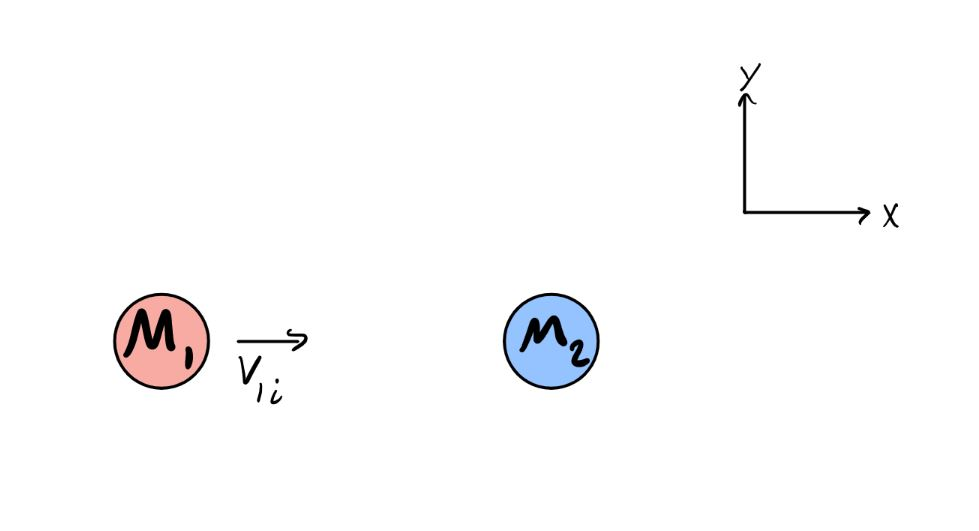
\includegraphics[height=4cm, width=7cm]{1.JPG}
  \end{center}

  Once the first ball hits the second ball, then they both go at different angles.

  \begin{center}
    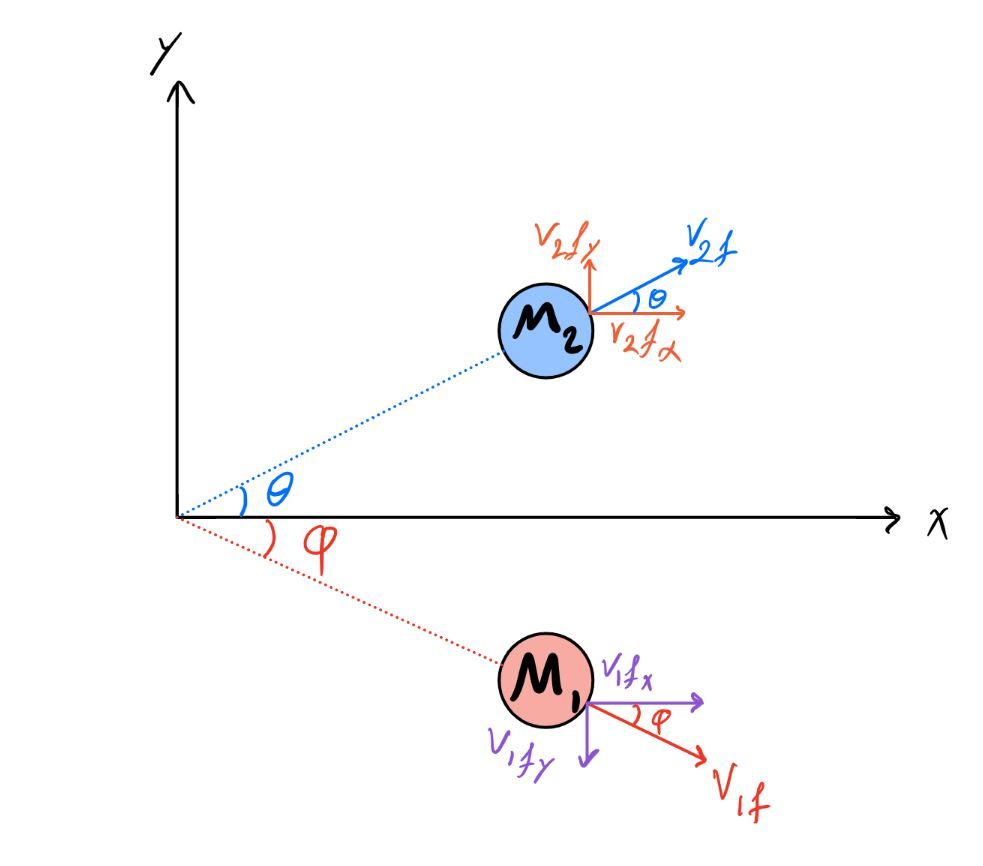
\includegraphics[height=8cm, width=10cm]{2.JPG}
  \end{center}

  \textbf{Elastic collision of balls with the same mass}

  \vspace{10px}

  Let's see how we can set up conservation of momentum. Since this is a elastic collision that means
  we also have conservation of kinetic energy.

  $
    \\
    \text{Momentum in the x-direction} ~~~ M_1 ~ v_{1i}=M_1 ~ v_{1f} ~ cos(\phi)+M_2 ~ v_{2f} ~ cos(\theta) ~~~~ (1)
    \\
    \\
    \text{Momentum in the y-direction} ~~~ 0=-M_1 ~ v_{1f} ~ sin(\phi)+M_2 ~ v_{2f} ~ sin(\theta) ~~~~~~~~~~~ (2)
  $

  \pagebreak

  Conservation of kinetic energy allows us to have:

  $
    \\
    \dfrac{1}{2} M_1 ~ v_{1i}^2=\dfrac{1}{2} M_1 ~ v_{1f}^2+\dfrac{1}{2} M_2 ~ v_{2f}^2 ~~~~~~~~ (3)
  $

  \vspace{10px}

  Assume the two balls have the same mass equals to $M_1=M_2=M$. Then we can rewrite equations $(1), (2),$ and $(3)$.

  $
    \\
    \begin{cases}
      v_{1i}=v_{1f} ~ cos(\phi)+v_{2f} ~ cos(\theta) ~~~~~~~~ (4)
      \\
      \\
      0=-v_{1f} sin(\phi)+v_{2f} ~ sin(\theta) ~~~~~~~~ (5)
      \\
      \\
      v_{1i}^2=v_{1f}^2+v_{2f}^2 ~~~~~~~~ (6)
    \end{cases}
    \\
    \\
  $

  Squaring $(4)$ and $(5)$ gives us:

  $
    \\
    \begin{cases}
      v_{1i}^2=v_{1f}^2 ~ cos^2(\phi)+v_{2f}^2 ~ cos^2(\theta)+2 v_{1f} ~ v_{2f} ~ cos(\phi) ~ cos(\theta) ~~~~~~~~ (7)
      \\
      \\
      0=v_{1f}^2 sin^2(\phi)+v_{2f}^2 ~ sin^2(\theta)-2 v_{1f} ~ v_{2f} ~ sin(\theta) ~ sin(\phi) ~~~~~~~~ (8)
    \end{cases}
    \\
    \\
  $

  By adding both equations $(7)$ and $(8)$ we get:

  $
    \\
    v_{1i}^2=v_{1f}^2 \left[sin^2(\phi)+cos^2(\phi)\right]+v_{2f}^2 \left[sin^2(\theta)+cos^2(\theta)\right]
    +2 v_{1f} ~ v_{2f} ~ \left[cos(\phi) ~ cos(\theta)-sin(\phi) ~ sin(\theta)\right]
    \\
    \\
    v_{1i}^2=v_{1f}^2+v_{2f}^2+2 v_{1f} ~ v_{2f} ~ \left[cos(\phi) ~ cos(\theta)-sin(\phi) ~ sin(\theta)\right]
    \\
    \\
  $

  Using $\boxed{cos(\phi+\theta)=cos(\phi) ~ cos(\theta)-sin(\phi) sin(\theta)}$ identity we have:

  $
    \\
    \\
    \therefore ~~~ v_{1i}^2=v_{1f}^2+v_{2f}^2+2 v_{1f} ~ v_{2f} ~ cos(\phi+\theta) ~~~~~~~~ (9)
    \\
    \\
  $

  From equations $(6)$ and $(9)$:

  $
    \\
    \begin{cases}
      v_{1i}^2=v_{1f}^2+v_{2f}^2+2 v_{1f} ~ v_{2f} ~ cos(\phi+\theta)
      \\
      \\
      v_{1i}^2=v_{1f}^2+v_{2f}^2
    \end{cases}
    \Longrightarrow
    v_{1f}^2+v_{2f}^2=v_{1f}^2+v_{2f}^2+2 v_{1f} ~ v_{2f} ~ cos(\theta+\phi)
    \\
    \\
    \\
    \therefore ~~~ \boxed{\theta+\phi=\dfrac{\pi}{2}} ~~~~ \checkmark
    \\
    \\
  $

 For a two dimensional collision where the balls have the same mass, \emph{billiard balls}, they always scatter 
 off at $\dfrac{\pi}{2}$ with each other. In other words, the angle between the two balls after the collision is
 always $\dfrac{\pi}{2}$ when they have the same mass.
 
 $
    \\
    \begin{cases}
      v_{1i}=v_{1f} ~ cos(\phi)+v_{2f} ~ cos(\theta) ~~~~~~~~ (4)
      \\
      \\
      0=-v_{1f} sin(\phi)+v_{2f} ~ sin(\theta) ~~~~~~~~ (5)
    \end{cases} 
    \Longrightarrow 
    \begin{cases}
      v_{1f}=\dfrac{
        \begin{vmatrix}
          v_{1i} & cos(\theta)
          \\
          0 & sin(\theta)
        \end{vmatrix}
      }{
        \begin{vmatrix}
          cos(\phi) & cos(\theta)
          \\
          -sin(\phi) & sin(\theta)
        \end{vmatrix}
      }
      \\
      \\
      v_{2f}=\dfrac{
        \begin{vmatrix}
          cos(\phi) & v_{1i}
          \\
          -sin(\phi) & 0
        \end{vmatrix}
      }{
        \begin{vmatrix}
          cos(\phi) & cos(\theta)
          \\
          -sin(\phi) & sin(\theta)
        \end{vmatrix}
      }
    \end{cases}
    \\
    \\
    \\
    \boxed{sin(\phi+\theta)=cos(\phi) ~ sin(\theta)+sin(\phi) ~ cos(\theta)}
    \\
    \\
    \\
    \therefore ~~~ \begin{cases}
      v_{1f}=v_{1i} \dfrac{sin(\theta)}{sin(\phi+\theta)}
      \\
      \\
      v_{2f}=v_{1i} \dfrac{sin(\phi)}{sin(\phi+\theta)}
    \end{cases} ~~~~ \checkmark
    \\
    \\
 $

 \vspace{20px}

\textbf{Elastic collision of balls with different masses}

\vspace{10px}

Let's study the case where the masses of the balls are not the same $M_1 \neq M_2$. Our case is an elastic collision
which means both momentum and kinetic energy are conserved. 

$
  \\
  \\
  \begin{cases}
    M_1 ~ v_{1i}=M_1 ~ v_{1f}+M_2 ~ v_{2f}  
    \\
    \\
    \dfrac{1}{2} M_1 ~ v_{1i}^2=\dfrac{1}{2} M_1 ~ v_{1f}^2+\dfrac{1}{2} M_2 ~ v_{2f}^2  
  \end{cases}
  \Longrightarrow 
  \begin{cases}
    M_1 ~ v_{1i}=M_1 ~ v_{1f}+M_2 ~ v_{2f}
    \\
    \\
    M_1 ~ v_{1i}^2=M_1 ~ v_{1f}^2+M_2 ~ v_{2f}^2
  \end{cases}
  \\
  \\
  \\
  \\
  \begin{cases}
    M_1 ~ v_{1i}-M_1 ~ v_{1f}=M_2 ~ v_{2f}
    \\
    \\
    M_1 ~ v_{1i}^2-M_1 ~ v_{1f}^2=M_2 ~ v_{2f}^2
  \end{cases}
  \Longrightarrow
  \begin{cases}
    M_1\left(v_{1i}-v_{1f}\right)=M_2 ~ v_{2f} ~~~~~~~~ (A)
    \\
    \\
    M_1 ~ \left(v_{1i}-v_{1f}\right) ~ \left(v_{1i}+v_{1f}\right)=M_2 ~ v_{2f}^2 ~~~~~~~~ (B)
  \end{cases}
  \\
  \\
$

Dividing $(A)$ and $(B)$ gives us $\dfrac{1}{v_{1i}+v_{1f}}=\dfrac{1}{v_{2f}} \Longrightarrow v_{1i}+v_{1f}=v_{2f} ~~~~~ (C)$.
Now we can eliminate $v_{2f}$ by substituting $(C)$ into equation $(A)$.

$
  \\
  M_1\left(v_{1i}-v_{1f}\right)=M_2 ~ v_{2f}
  \Longrightarrow
  M_1\left(v_{1i}-v_{1f}\right)=M_2 ~ \left[v_{1i}+v_{1f}\right]
  \\
  \\
  M_1 ~ v_{1i}-M_1 ~ v_{1f}=M_2 ~ v_{1i}+M_2 ~ v_{1f} 
  \Longrightarrow 
  M_1 ~ v_{1i}-M_2 ~ v_{1i}=M_1 ~ v_{1f}+M_2 ~ v_{1f}
  \\
  \\
  \\
  \therefore ~~~ \boxed{v_{1f}=v_{1i} ~ \dfrac{M_1 - M_2}{M_1+M_2}} ~~~~ \checkmark
  \\
  \\
$

Time to eliminate $v_{1f}$, again by using $(C)$ and $(A)$. So we have

$
  \\
  M_1\left(v_{1i}-v_{1f}\right)=M_2 ~ v_{2f} 
  \Longrightarrow  M_1 \left[v_{1i}-\left(v_{2f}-v_{1i}\right)\right]=M_2 ~ v_{2f}
  \\
  \\
  M_1 \left[2v_{1i}-v_{2f}\right]=M_2 ~ v_{2f} \Longrightarrow 2 M_1 ~ v_{1i}=M_1 ~ v_{2f}+M_2 ~ v_{2f}
  \\
  \\
  \\
  \therefore ~~~ \boxed{v_{2f}=2 v_{1i} \dfrac{M_1}{M_1+M_2}} ~~~~ \checkmark
  \\
  \\
$

\pagebreak

We would like to know when the energy of the second ball is the largest. We are trying to find the maximum amount 
of kinetic energy of the first ball of mass $M_1$ which we can transfer to the second ball of mass $M_2$. We are considering 
the maximum kinetic energy of the first ball to be transferred to the second ball. By conservation of energy and momentum we have

$
  \\
  \begin{cases}
    M_1 ~ v_{1i}=M_1 ~ v_{1f}+M_2 ~ v_{2f}  
    \\
    \\
    \dfrac{1}{2} M_1 ~ v_{1i}^2=\dfrac{1}{2} M_1 ~ v_{1f}^2+\dfrac{1}{2} M_2 ~ v_{2f}^2  
  \end{cases}
  \\
  \\
$

When $v_{1f}=0$, then $100\%$ of the kinetic energy of the first ball must be transferred to the second ball in our case 
which is an elastic collision.

$
  \\
  \begin{cases}
    M_1 ~ v_{1i}=0+M_2 ~ v_{2f}  
    \\
    \\
    M_1 ~ v_{1i}^2=0+M_2 ~ v_{2f}^2  
  \end{cases} 
  \Longrightarrow 
  \left(\dfrac{M_1}{M_2} v_{1i} \right)^2=\dfrac{M_1}{M_2} v_{1i}^2
  \Longrightarrow \dfrac{M_1}{M_2}=1
  \\
  \\
  \\
  \therefore ~~~ \boxed{M_1=M_2} ~~~~ \checkmark
  \\
$

\pagebreak

\textbf{Non-head-on elastic collision of balls with different masses (1)}

\vspace{10px}

A head-on collision is a traffic collision where the front ends of two vehicles such as cars, trains, ships or planes 
hit each other when travelling in opposite directions, as opposed to a side collision or rear-end collision.
A head on collision means that the point of impact is on the straight line connecting the center of gravity of each of 
the objects. The centres of mass of the two bodies should be travelling in the same straight line and approaching each other 
to call it a head on collision.

\begin{center}
  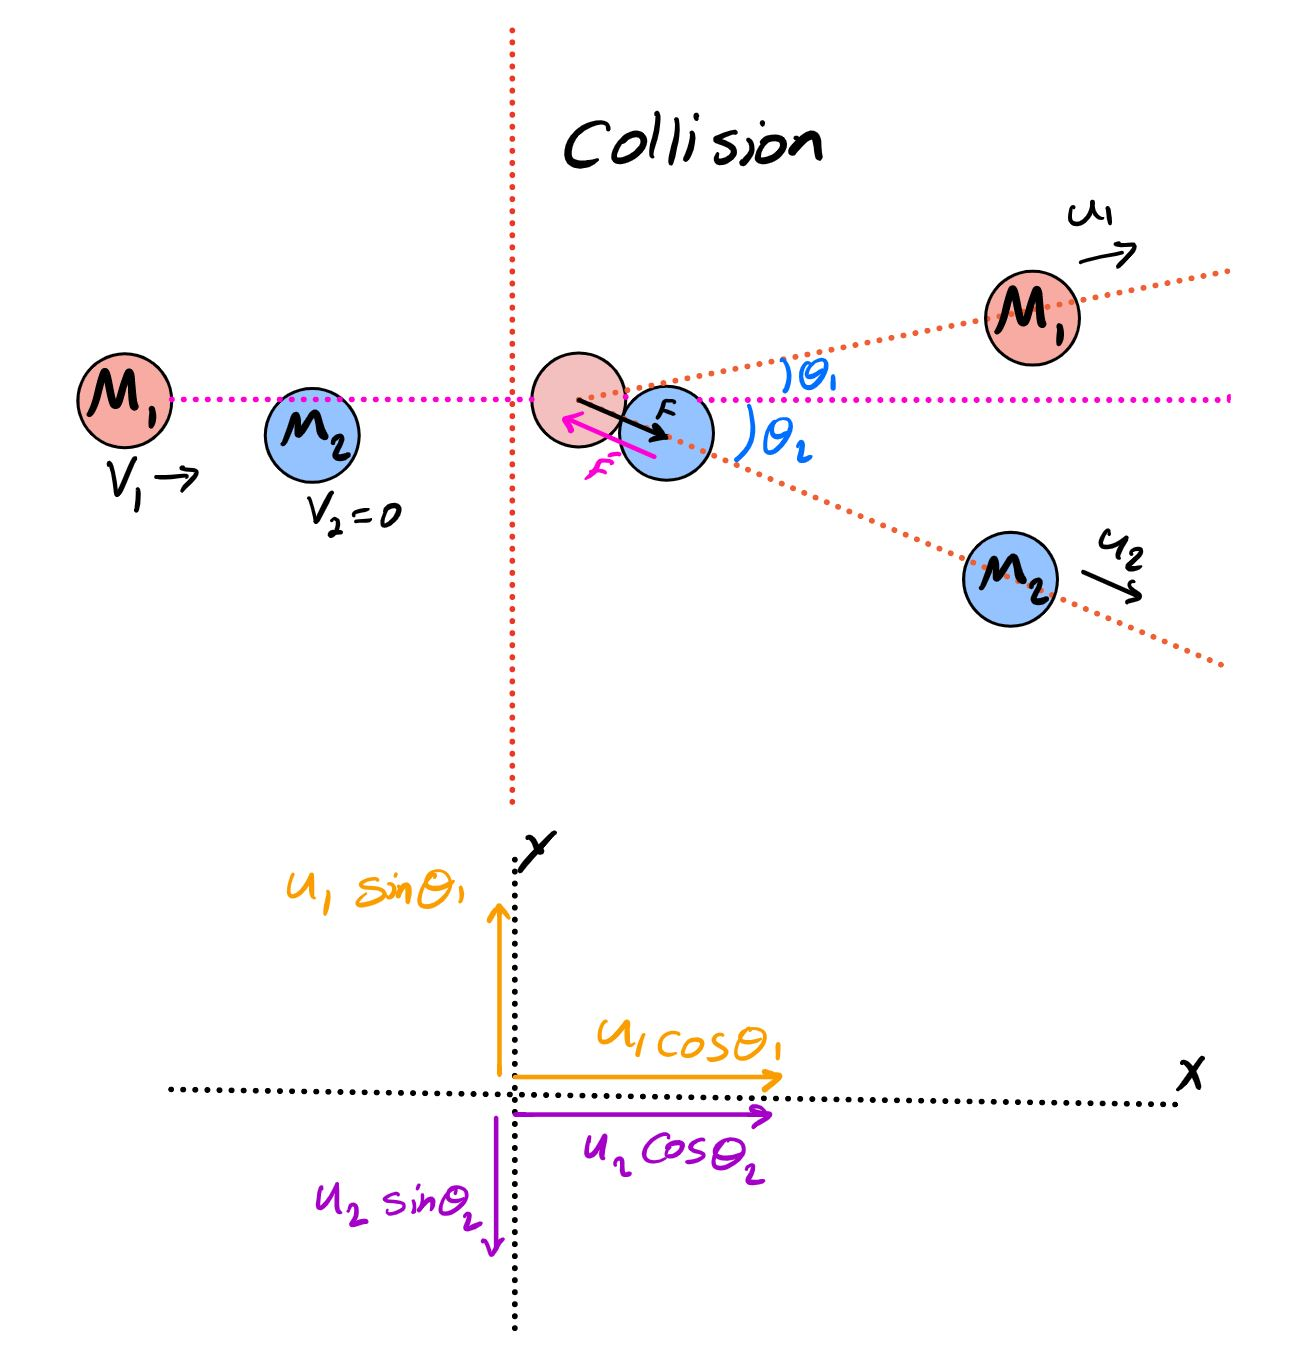
\includegraphics[height=11cm, width=10cm]{3.JPG}
\end{center}

$
  \\
  \text{Momentum in the x-direction (conserved)} ~~~ (I): ~~~ m_1 ~ v_{1}+0=m_1 ~ u_1 ~ cos(\theta_1)+m_2 ~ u_2 ~ cos(\theta_2)
  \\
  \\
  \text{Momentum in the y-direction (conserved)} ~~~ (II): ~~~ 0=m_1 ~ u_1 ~ sin(\theta_1)-m_2 ~ u_2 ~ sin(\theta_2)
  \\
  \\
  \text{Kinetic energy (conserved and scalar quantity)} ~~~ (III): 
  \dfrac{1}{2} m_1 ~ v^2_1+0=\dfrac{1}{2} m_1 ~ u^2_1+\dfrac{1}{2} m_2 ~ u^2_2
$

\vspace{10px}

We have got three equations meaning we only can find 3 unknown variables. Assuming we are given 
$m_1, m_2, v_1,$ and $u_1$ we can find $u_2, ~ \theta_1,$ and $\theta_2$. From equation $(III)$ we have

$
  \\
  m_1 ~ v^2_1=m_1 ~ u^2_1+m_2 ~ u^2_2
  \\
  \\
  \therefore ~~~ \dfrac{m_1}{m_2} \left(v_1^2-u_1^2\right)=u_2^2
  \\
  \\
  \\
  \therefore ~~~ \boxed{u_2=\sqrt{\dfrac{m_1}{m_2} \left(v_1^2-u_1^2\right)}} ~~~~ \checkmark
  \\
  \\
  \\
$

Now that we have $u_2$, we are able to find $\theta_1$ and $\theta_2$.

$
\\
  (IV): ~~~ \begin{cases}
    m_1 ~ u_1 ~ cos(\theta_1)+m_2 ~ u_2 ~ cos(\theta_2)=m_1 ~ v_{1}
    \\
    \\
    m_1 ~ u_1 ~ sin(\theta_1)-m_2 ~ u_2 ~ sin(\theta_2)=0
  \end{cases}
  \\
  \\
$

Squaring and summing $(IV)$ gives us

$
  \\
  \\
  m_1^2 ~ u_1^2 \left[cos^2(\theta_1)+sin^2(\theta_1)\right]=m_2^2 ~ u_2^2 ~ sin^2(\theta_2)
  +\left[m_1^2 ~ v_1^2+m_2^2 ~ u_2^2 ~ cos^2(\theta_2)-2m_1 ~ v_1 ~ m_2 ~ u_2 ~ cos(\theta_2)\right]
  \\
  \\
  m_1^2 ~ u_1^2=m_2^2 ~ u_2^2 ~ sin^2(\theta_2)+m_1^2 ~ v_1^2 +m_2^2 ~ u_2^2 ~ cos^2(\theta_2)-2m_1 ~ v_1 ~ m_2 ~ u_2 ~ cos(\theta_2)
  \\
  \\
  m_1^2 ~ u_1^2=m_2^2 ~ u_2^2 \left[sin^2(\theta_2)+cos^2(\theta_2)\right]+m_1^2 ~ v_1^2-2m_1 ~ v_1 ~ m_2 ~ u_2 ~ cos(\theta_2)
  \\
  \\
  m_1^2 ~ u_1^2=m_2^2 ~ u_2^2+m_1^2 ~ v_1^2-2m_1 ~ v_1 ~ m_2 ~ u_2 ~ cos(\theta_2)
  \\
  \\
  cos(\theta_2)=\dfrac{
    -m_1^2 ~ u_1^2+m_2^2 ~ u_2^2+m_1^2 ~ v_1^2 
  }{
    2 ~ m_1 ~ v_1 ~ m_2 ~ u_2
  }=\dfrac{
    m_1^2 ~ \left(v_1^2-u_1^2\right)+m_2^2 ~u_2^2 
  }{
    2 m_1 ~ m_2 ~ v_1 ~ u_2
  }
  \\
  \\
  \\
  \therefore ~~~ \boxed{
    \theta_2=cos^{-1}\left[
      \dfrac{
        m_1^2 ~ \left(v_1^2-u_1^2\right)+m_2^2 ~u_2^2 
      }{
        2 m_1 ~ m_2 ~ v_1 ~ u_2
      }
    \right]
  } ~~~~ \checkmark
$

\pagebreak

Using the same method as we used above to calculate $\theta_1$

$
  \\
  \\
  (IV): ~~~ \begin{cases}
    m_1 ~ u_1 ~ cos(\theta_1)+m_2 ~ u_2 ~ cos(\theta_2)=m_1 ~ v_{1}
    \\
    \\
    m_1 ~ u_1 ~ sin(\theta_1)-m_2 ~ u_2 ~ sin(\theta_2)=0
  \end{cases}
  \\
  \\
  \\
  \begin{cases}
    m_1 ~ u_1 ~ cos(\theta_1)-m_1 ~ v_{1}=-m_2 ~ u_2 ~ cos(\theta_2)
    \\
    \\
    m_1 ~ u_1 ~ sin(\theta_1)=m_2 ~ u_2 ~ sin(\theta_2)
  \end{cases}
  \\
  \\
  \\
  \begin{cases}
    m_1^2 ~ u_1^2 ~ cos^2(\theta_1)+m_1^2 ~ v_{1}^2-2 ~ m_1 ~ u_1 ~ m_1 ~ v_1 ~ cos(\theta_1)=m_2^2 ~ u_2^2 ~ cos^2(\theta_2)
    \\
    \\
    m_1^2 ~ u_1^2 ~ sin^2(\theta_1)=m_2^2 ~ u_2^2 ~ sin^2(\theta_2)
  \end{cases}
  \\
  \\
  \\
  m_1^2 ~ u_1^2 ~ cos^2(\theta_1)+m_1^2 ~ v_{1}^2-2 ~ m_1 ~ u_1 ~ m_1 ~ v_1 ~ cos(\theta_1)
  +m_1^2 ~ u_1^2 ~ sin^2(\theta_1)
  =m_2^2 ~ u_2^2 ~ cos^2(\theta_2)+m_2^2 ~ u_2^2 ~ sin^2(\theta_2)
  \\
  \\
  \\
  m_1^2 ~ u_1^2 ~ \left[cos^2(\theta_1)+sin^2(\theta_1)\right]+m_1^2 ~ v_1^2-2 ~ m_1 ~ u_1 ~ m_1 ~ v_1 ~ cos(\theta_1)
  =m_2^2 ~ u_2^2 ~ \left[cos^2(\theta_2)+sin^2(\theta_2)\right]
  \\
  \\
  \\
  m_1^2 ~ u_1^2+m_1^2 ~ v_1^2-2 ~ m_1 ~ u_1 ~ m_1 ~ v_1 ~ cos(\theta_1)
  =m_2^2 ~ u_2^2
  \\
  \\
  \\
  2 ~ m_1 ~ u_1 ~ m_1 ~ v_1 ~ cos(\theta_1)=m_1^2 ~ u_1^2+m_1^2 ~ v_1^2-m_2^2 ~ u_2^2
  \\
  \\
  \\
  cos(\theta_1)=\dfrac{m_1^2 \left(u_1^2+v_1^2\right)-m_2^2 ~ u_2^2}{2 ~ m_1^2 ~ u_1 ~ v_1}
  \\
  \\
  \\
  \therefore ~~~ \boxed{
    \theta_1=cos^{-1} \left[
      \dfrac{m_1^2 \left(u_1^2+v_1^2\right)-m_2^2 ~ u_2^2}{2 ~ m_1^2 ~ u_1 ~ v_1}
    \right]
  } ~~~~ \checkmark
  \\
  \\
$

Note: The domain and range of $y=cos^{-1}(x)$ are $-1 \leq x \leq +1$ and $0 \leq y \leq +\pi$. 

We know the kinetic energy of the second ball is 
$
  \\
  \\
  KE=\dfrac{1}{2} ~ m_2 ~ u_2^2=\dfrac{1}{2} ~ m_2 ~ \left[
    \sqrt{\dfrac{m_1}{m_2} \left(v_1^2-u_1^2\right)}
  \right]^2
  =\dfrac{1}{2} ~ m_2 ~ \dfrac{m_1}{m_2} \left(v_1^2-u_1^2\right)
  \\
  \\
  \\
  \therefore ~~~ \boxed{
    KE=\dfrac{1}{2} ~ m_1 \left(v_1^2-u_1^2\right)
  } ~~~~ \checkmark
  \\
  \\
$

Maximizing the energy transferred to the second ball? (Largest kinetic energy)

\vspace{10px}

\textbf{Some examples}

\vspace{10px}

$
  (A) ~ m_1=m_2=2 ~ kg, v_1=3 ~ m/s ~ , u_1=2 ~ m/s
  \\
  \\
  \begin{cases}
    u_2=\sqrt{\dfrac{m_1}{m_2} \left(v_1^2-u_1^2\right)}=\sqrt{\left(v_1^2-u_1^2\right)}=2.2360 ~ m/s
    \\
    \\
    \theta_1=cos^{-1} \left[
      \dfrac{m_1^2 \left(u_1^2+v_1^2\right)-m_2^2 ~ u_2^2}{2 ~ m_1^2 ~ u_1 ~ v_1}
    \right]=48.1896^{\circ}
    \\
    \\
    \theta_2=cos^{-1}\left[
      \dfrac{
        m_1^2 ~ \left(v_1^2-u_1^2\right)+m_2^2 ~u_2^2 
      }{
        2 m_1 ~ m_2 ~ v_1 ~ u_2
      }
    \right]=41.8103^{\circ}
  \end{cases} ~~~ \therefore ~~~ \boxed{\theta_1+\theta_2=\dfrac{\pi}{2}} ~~~~ \checkmark 
  \\
  \\
  \\
  (B) ~ m_1>m_2, ~ 5 ~ kg, ~ 4 ~ kg, ~ v_1=4 ~ m/s ~ , u_1=2 ~ m/s
  \\
  \\
  \begin{cases}
    u_2=\sqrt{\dfrac{m_1}{m_2} \left(v_1^2-u_1^2\right)}=3.8729 ~ m/s
    \\
    \\
    \theta_1=cos^{-1} \left[
      \dfrac{m_1^2 \left(u_1^2+v_1^2\right)-m_2^2 ~ u_2^2}{2 ~ m_1^2 ~ u_1 ~ v_1}
    \right]=49.4583^{\circ}
    \\
    \\
    \theta_2=cos^{-1}\left[
      \dfrac{
        m_1^2 ~ \left(v_1^2-u_1^2\right)+m_2^2 ~u_2^2 
      }{
        2 m_1 ~ m_2 ~ v_1 ~ u_2
      }
    \right]=29.3757^{\circ}
  \end{cases} 
  \\
  \\
  \\
  (C) ~ m_1<m_2, ~ 2 ~ kg, ~ 6 ~ kg, ~ v_1=2 ~ m/s ~ , u_1=1 ~ m/s
  \\
  \\
  \begin{cases}
    u_2=\sqrt{\dfrac{m_1}{m_2} \left(v_1^2-u_1^2\right)}=1 ~ m/s
    \\
    \\
    \theta_1=cos^{-1} \left[
      \dfrac{m_1^2 \left(u_1^2+v_1^2\right)-m_2^2 ~ u_2^2}{2 ~ m_1^2 ~ u_1 ~ v_1}
    \right]=180^{\circ}
    \\
    \\
    \theta_2=cos^{-1}\left[
      \dfrac{
        m_1^2 ~ \left(v_1^2-u_1^2\right)+m_2^2 ~u_2^2 
      }{
        2 m_1 ~ m_2 ~ v_1 ~ u_2
      }
    \right]=0^{\circ} 
  \end{cases}
$

\pagebreak

\textbf{Non-head-on elastic collision of balls with different masses (2)}

\vspace{10px}

A head-on collision is a traffic collision where the front ends of two vehicles such as cars, trains, ships or planes 
hit each other when travelling in opposite directions, as opposed to a side collision or rear-end collision.
A head on collision means that the point of impact is on the straight line connecting the center of gravity of each of 
the objects. The centres of mass of the two bodies should be travelling in the same straight line and approaching each other 
to call it a head on collision.

\begin{center}
  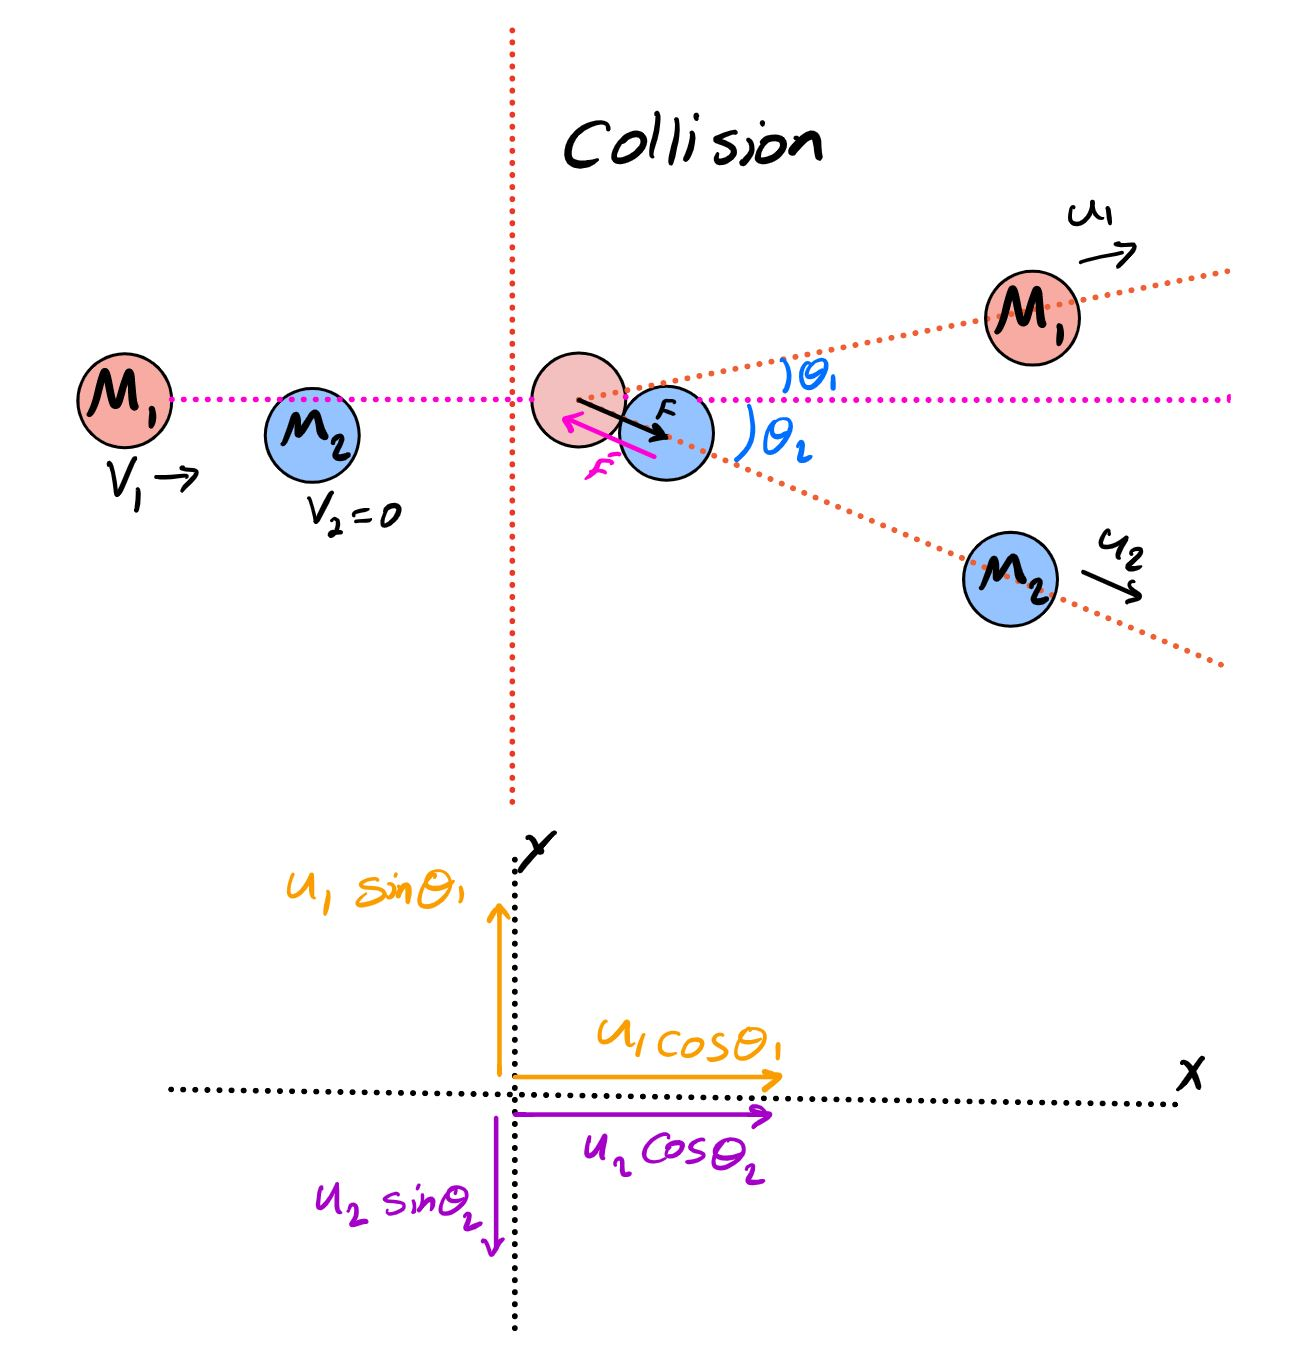
\includegraphics[height=11cm, width=10cm]{3.JPG}
\end{center}

$
  \\
  \text{Momentum in the x-direction (conserved)} ~~~ (I): ~~~ m_1 ~ v_{1}+0=m_1 ~ u_1 ~ cos(\theta_1)+m_2 ~ u_2 ~ cos(\theta_2)
  \\
  \\
  \text{Momentum in the y-direction (conserved)} ~~~ (II): ~~~ 0=m_1 ~ u_1 ~ sin(\theta_1)-m_2 ~ u_2 ~ sin(\theta_2)
  \\
  \\
  \text{Kinetic energy (conserved and scalar quantity)} ~~~ (III): 
  \dfrac{1}{2} m_1 ~ v^2_1+0=\dfrac{1}{2} m_1 ~ u^2_1+\dfrac{1}{2} m_2 ~ u^2_2
$

\vspace{10px}

Assuming we are given $m_1, m_2, v_1,$ and $\theta_2$. We can find $u_1, ~ u_2$, and $\theta_1$. 
Let's define \textcolor{red}{$sin(\theta_2) \equiv \mathbf{S}$ and $cos(\theta_2) \equiv \mathbf{C}$}.

\vspace{10px}

$
  \begin{cases}
    (1): ~ m_1 ~ u_1 ~ cos(\theta_1)+m_2 ~ u_2 ~ cos(\theta_2)=m_1 ~ v_{1}
    \\
    \\
    (2): ~ m_1 ~ u_1 ~ sin(\theta_1)-m_2 ~ u_2 ~ sin(\theta_2)=0
    \\
    \\
    (3): ~ m_1 ~ v^2_1=m_1 ~ u^2_1+m_2 ~ u^2_2 
  \end{cases}
  \\
  \\
  \\
  \text{From} ~ (3) ~~ \therefore ~~~ \boxed{
    \begin{cases}
      (4): ~ u^2_1=v^2_1-\dfrac{m_2}{m_1} ~ u^2_2
      \\
      \\
      (5): ~ v^2_1=u^2_1+\dfrac{m_2}{m_1} ~ u^2_2
    \end{cases}
  } ~~~~ \checkmark
  \\
  \\
  \\
$

Squaring and summing $(1)$ and $(2)$ gives us:

\vspace{10px}

$
  \begin{cases}
    m^2_1 ~ u^2_1 ~ cos^2(\theta_1)+m^2_2 ~ u^2_2 ~ cos^2(\theta_2)+2 m_1 ~ m_2 ~ u_1 ~ u_2 ~ cos(\theta_1) ~ cos(\theta_2)=m^2_1 ~ v^2_{1}
    \\
    \\
    m^2_1 ~ u^2_1 ~ sin^2(\theta_1)+m^2_2 ~ u^2_2 ~ sin^2(\theta_2)-2 m_1 ~ m_2 ~ u_1 ~ u_2 ~ sin(\theta_1) ~ sin(\theta_2)=0
  \end{cases}
  \\
  \\
  \rule{13cm}{1pt}
  \\
  \\
  m^2_1 ~ u^2_1 \left[cos^2(\theta_1)+sin^2(\theta_1)\right]
  +m^2_2 ~ u^2_2 \left[cos^2(\theta_2)+sin^2(\theta_2)\right]
  \\
  \\
  +2 m_1 ~ m_2 ~ u_1 ~ u_2 ~ \left[cos(\theta_1) ~ cos(\theta_2)-sin(\theta_1) ~ sin(\theta_2)\right]
  =m^2_1 ~ v^2_{1}
  \\
  \\
  \\
  m^2_1 ~ u^2_1+m^2_2 ~ u^2_2 
  +2 m_1 ~ m_2 ~ u_1 ~ u_2 ~ \left[cos(\theta_1) ~ cos(\theta_2)-sin(\theta_1) ~ sin(\theta_2)\right]
  =m^2_1 ~ v^2_{1}
  \\
  \\
$

Let's define \textcolor{red}{$cos(\theta_1) ~ cos(\theta_2)-sin(\theta_1) ~ sin(\theta_2) \equiv ~ \mathbf{K}$}
and from $(5)$ we have the following.

\vspace{10px}

$
  \\
  m^2_1 ~ u^2_1+m^2_2 ~ u^2_2 
  +2 m_1 ~ m_2 ~ u_1 ~ u_2 ~ \textcolor{red}{\mathbf{K}}
  =m^2_1 ~ v^2_{1}
  \\
  \\
  \\
  m^2_1 ~ u^2_1+m^2_2 ~ u^2_2+2 m_1 ~ m_2 ~ u_1 ~ u_2 ~ \textcolor{red}{\mathbf{K}}=m^2_1 \left[u^2_1+\dfrac{m_2}{m_1} ~ u^2_2\right]
  \\
  \\
  \\
  m^2_1 ~ u^2_1+m^2_2 ~ u^2_2+2 m_1 ~ m_2 ~ u_1 ~ u_2 ~ \textcolor{red}{\mathbf{K}}=m^2_1 ~ u^2_1+m_1 ~ m_2 ~ u^2_2
  \\
  \\
  \\
  m^2_2 ~ u^2_2+2 m_1 ~ m_2 ~ u_1 ~ u_2 ~ \textcolor{red}{\mathbf{K}}=m_1 ~ m_2 ~ u^2_2
  \\
  \\
  \\
  2 m_1 ~ m_2 ~ u_1 ~ u_2 ~ \textcolor{red}{\mathbf{K}}=u^2_2 \left[m_1 ~ m_2-m^2_2\right]
  \\
  \\
  \\
  2 m_1 ~ m_2 ~ u_1 ~ \textcolor{red}{\mathbf{K}}=u_2 \left[m_1 ~ m_2-m^2_2\right]
  \\
  \\
  \\
  u_2=\dfrac{2 m_1 ~ m_2 ~ u_1 ~ \textcolor{red}{\mathbf{K}}}{m_1 ~ m_2-m^2_2}
  =\dfrac{2 m_1 ~ m_2 ~ u_1 ~ \textcolor{red}{\mathbf{K}}}{m_2 \left(m_1-m_2\right)}
  \\
  \\
  \\
  \therefore ~~~ \boxed{
    (6): ~ u_2=\dfrac{2m_1 ~ u_1 ~ \textcolor{red}{\mathbf{K}}}{m_1-m_2}
  } ~~~~ \checkmark
  \\
  \\
  \\
  \therefore ~~~ \dfrac{u_2}{u_1}=\dfrac{2m_1 ~ \textcolor{red}{\mathbf{K}}}{m_1-m_2}
  \\
  \\
  \\
  \text{Squaring $(6)$ and plugging in $(4)$}
  \\
  \\
  \\
  \left(\dfrac{u_2}{u_1}\right)^2=\dfrac{\left(2m_1 ~ \textcolor{red}{\mathbf{K}}\right)^2}{\left(m_1-m_2\right)^2}
  \\
  \\
  \\
  u^2_2 ~ \left(m_1-m_2\right)^2=4 m^2_1 ~ \textcolor{red}{\mathbf{K}^2} ~ u_1
  =4 m^2_1 ~ \textcolor{red}{\mathbf{K}^2} ~ \left(v^2_1-\dfrac{m_2}{m_1} ~ u^2_2\right)
  \\
  \\
  \\
  u^2_2 ~ \left(m_1-m_2\right)^2
  =4 m^2_1 ~ \textcolor{red}{\mathbf{K}^2} ~ v^2_1-4 m_1 ~ m_2 ~ \textcolor{red}{\mathbf{K}^2} ~ u^2_2
  \\
  \\
  \\
  u^2_2 \left[\left(m_1-m_2\right)^2+4m_1 ~ m_2 ~ \textcolor{red}{\mathbf{K}^2} \right]=4 m^2_1 ~ \textcolor{red}{\mathbf{K}^2} ~ v^2_1
  \\
  \\
  \\
  u^2_2=\dfrac{4 m^2_1 ~ \textcolor{red}{\mathbf{K}^2} ~ v^2_1}{\left(m_1-m_2\right)^2+4 m_1 ~ m_2 ~ \textcolor{red}{\mathbf{K}^2}}
  \\
  \\
  \\
  u_2=\dfrac{
    2 m_1 ~ \textcolor{red}{\mathbf{K}} ~ v_1
  }{
    \sqrt{\left(m_1-m_2\right)^2+4 m_1 ~ m_2 ~ \textcolor{red}{\mathbf{K}^2}}
  }
  \\
  \\
  \\
  \therefore ~~~ \boxed{
    u_2=\dfrac{
      2 m_1 ~ v_1 ~ \left[cos(\theta_1) ~ \textcolor{red}{\mathbf{C}}-sin(\theta_1) ~ \textcolor{red}{\mathbf{S}}\right]
    }{
      \sqrt{\left(m_1-m_2\right)^2+4 m_1 ~ m_2 ~ \left[cos(\theta_1) ~ \textcolor{red}{\mathbf{C}}-sin(\theta_1) ~ \textcolor{red}{\mathbf{S}}\right]^2}
    }
  } ~~~~ \checkmark
$

\end{document}
